
\documentclass[letterpaper,12pt,]{article}

\title{Take Home Essay}

\author{
        Doug Shi-Dong 260466662 \\
        SOCI 312 - Sociology of Work and Industry\\
        McGill University
}
\date{April 10, 2015}


\usepackage{titling}

\setlength{\droptitle}{5in}   % This is your set screw

\usepackage[%
    left=1in,%
    right=1in,%
    top=1in,%
    bottom=1.0in,%
    paperheight=11in,%
    paperwidth=8.5in%
]{geometry}%
\usepackage{comment}

\usepackage{listings}
\usepackage{graphicx}
\usepackage{amsmath}
\usepackage[section]{placeins}
\usepackage[font=small,skip=-2pt]{caption}
\usepackage{subcaption}

\lstdefinestyle{mystyle}{
    %backgroundcolor=\color{backcolour},   
    %commentstyle=\color{codegreen},
    %keywordstyle=\color{magenta},
    %numberstyle=\tiny\color{codegray},
    %stringstyle=\color{codepurple},
    basicstyle=\footnotesize,
    breakatwhitespace=false,         
    breaklines=true,                 
    captionpos=b,                    
    keepspaces=true,                 
    numbers=left,                    
    numberstyle=\footnotesize,               
    stepnumber=1,
    numbersep=5pt,
    showspaces=false,                
    showstringspaces=false,
    showtabs=false,                  
    tabsize=2,
    frame=single
}
\lstset{frame=single}

\pagestyle{empty} % Remove page numbering
\linespread{1.5} % Line Spacing

\begin{document}
\begin{titlepage}

\newcommand{\HRule}{\rule{\linewidth}{0.5mm}} % Defines a new command for the horizontal lines, change thickness here

\center % Center everything on the page
 
%----------------------------------------------------------------------------------------
%	HEADING SECTIONS
%----------------------------------------------------------------------------------------


\textsc{\LARGE McGill University}\\[3.5cm]
\textsc{\Large Numerical Analysis}\\[0.5cm] 
\textsc{\large MATH 578}\\[2.5cm]

%----------------------------------------------------------------------------------------
%	TITLE SECTION
%----------------------------------------------------------------------------------------

{ \huge \bfseries Homework 4 and 5}\\[1.5cm] % Title of your document

\HRule \\[0.4cm]
%----------------------------------------------------------------------------------------
%	AUTHOR SECTION
%----------------------------------------------------------------------------------------

\begin{minipage}{0.4\textwidth}
\begin{flushleft} \large
\emph{Name:}\\
Doug \textsc{Shi-Dong} % Your name
\end{flushleft}
\end{minipage}
~
\begin{minipage}{0.4\textwidth}
\begin{flushright} \large
\emph{Student ID:} \\
260466662\\
\end{flushright}
\end{minipage}\\[4cm]

\vfill{}
{\large November 17, 2015}\\[2cm]

\end{titlepage}

\section*{Question 10}

The trajectories are plotted in Figures \ref{fig:x1},\ref{fig:x2}. Notice that the Forward-Euler (FE) is not stable in both cases. The amplitude of the trajectories increase over time for FE. On the other hand, Backward-Euler (BE) seems to have a damping mechanism, decreasing the amplitude of the trajectories over time. Crank-Nicolson is neither unstable nor dissipative. A comparison of the amplitude is seen in Figure \ref{fig:r1} and \ref{fig:r2}.

Solving the second ODE with FE and BE exhibits an interesting behavior. The FE method has a greater frequency than the exact solution, whereas the BE method has a smaller frequency. Therefore, both methods cause time dilation of the solution. Crank-Nicolson is once again the same as the MATLAB computed solution.


\begin{figure}[h]
    \centering
    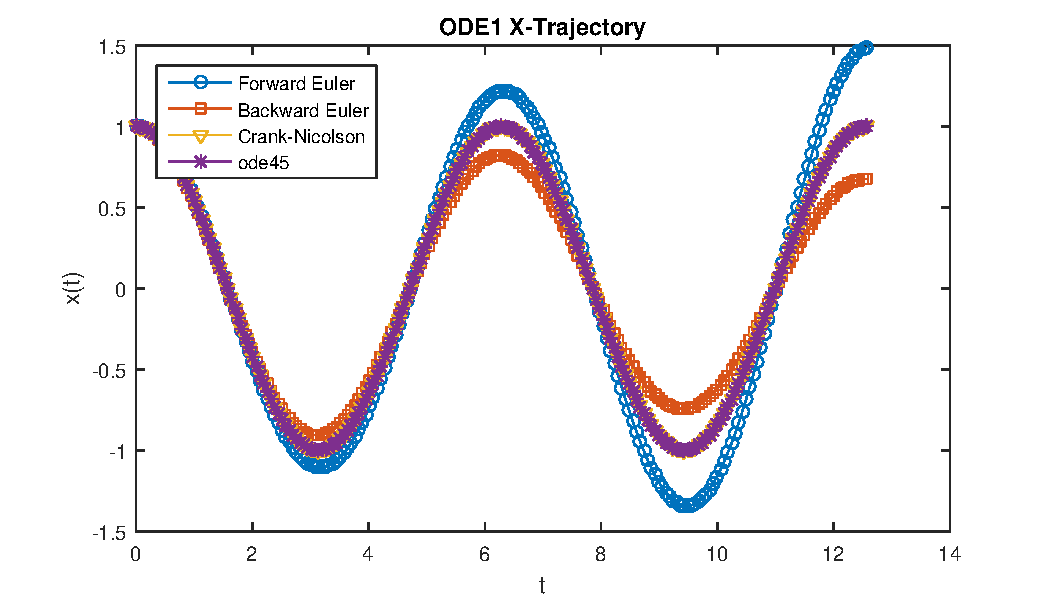
\includegraphics[height=0.4\textheight]{XTraj1}
    \caption{X Trajectory of ODE 1}
    \label{fig:x1}
\end{figure}

\begin{figure}
    \centering
    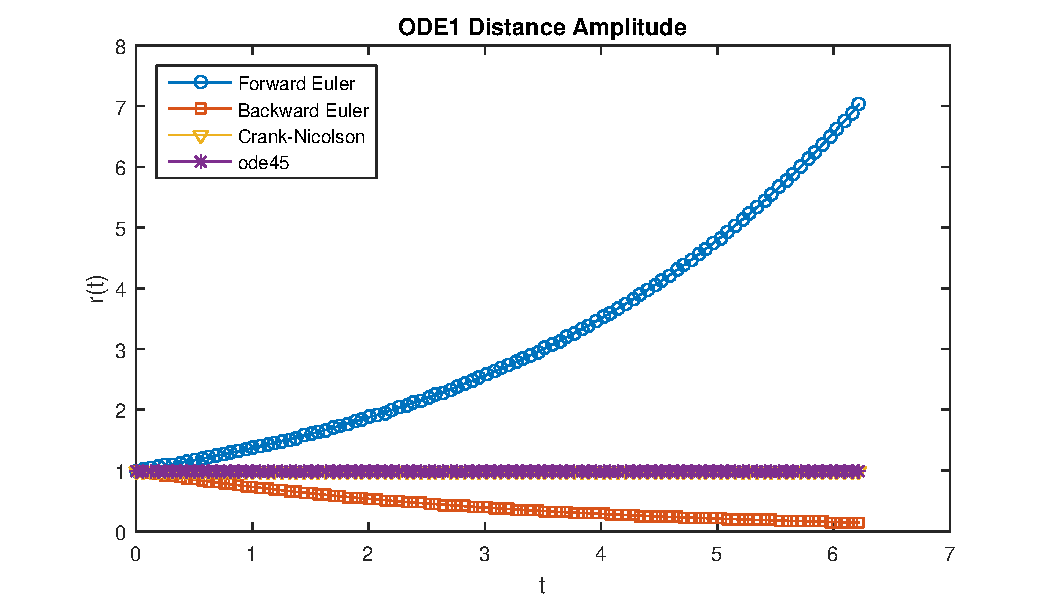
\includegraphics[height=0.4\textheight]{R1}
    \caption{Trajectory Amplitude of ODE 1}
    \label{fig:r1}
\end{figure}

\begin{figure}
    \centering
    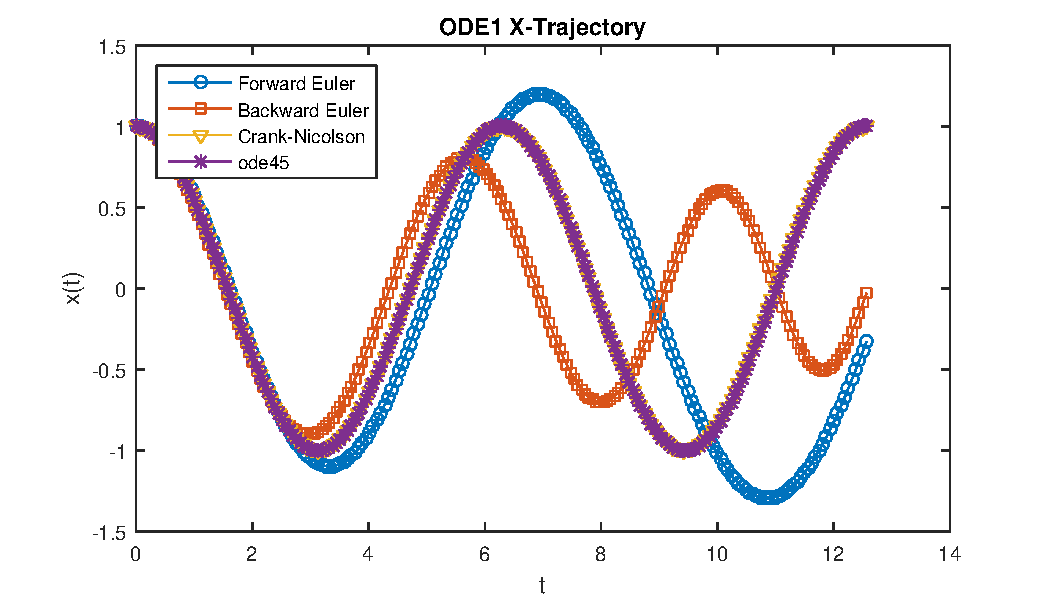
\includegraphics[height=0.4\textheight]{XTraj2}
    \caption{X Trajectory of ODE 2}
    \label{fig:x2}
\end{figure}

\begin{figure}
    \centering
    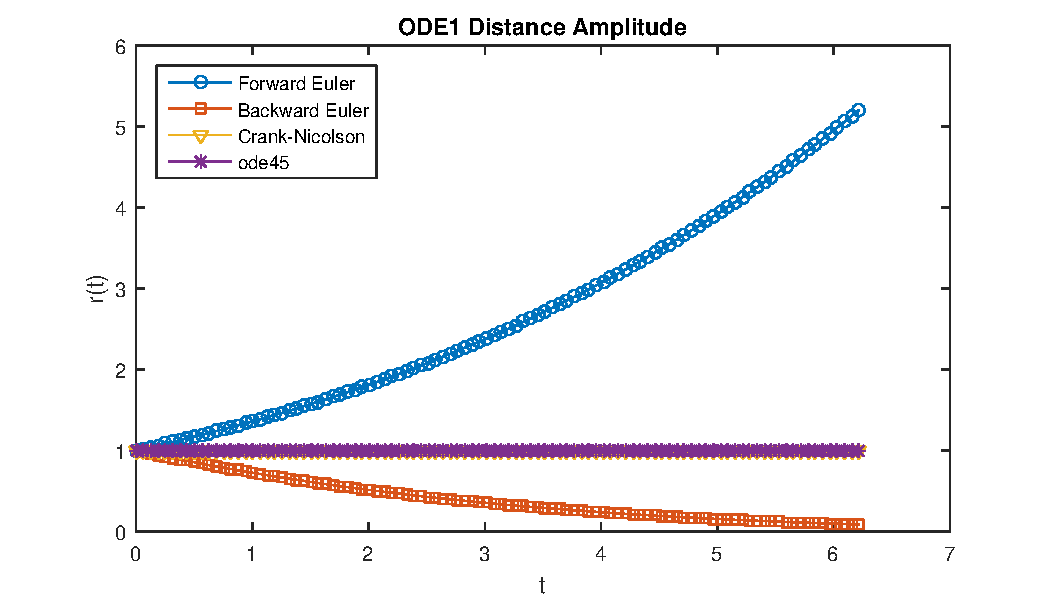
\includegraphics[height=0.4\textheight]{R2}
    \caption{Trajectory Amplitude of ODE 2}
    \label{fig:r2}
\end{figure}

\section*{Question 11}

The polynomial is evaluated using CVX for $p = [1, 1.5, 2, 4, 8, inf]$. The maximum error between the exact polynomial and the evaluated polynomial is then recorded and plotted in Figure \ref{fig:q11}. As expected, using the infinity-norm reduces the maximum error.

\section*{Question 12}

The results from CVX confirm the ones found by hand. CVX found $x = 1.6236e-12$ and $x = 1.3659e-09$ for the infinity-norm and two-norm respectively. The plot output is seen in Figure \ref{fig:q12}.

\begin{figure}[ht]
\begin{minipage}[b]{0.45\linewidth}
    \centering
    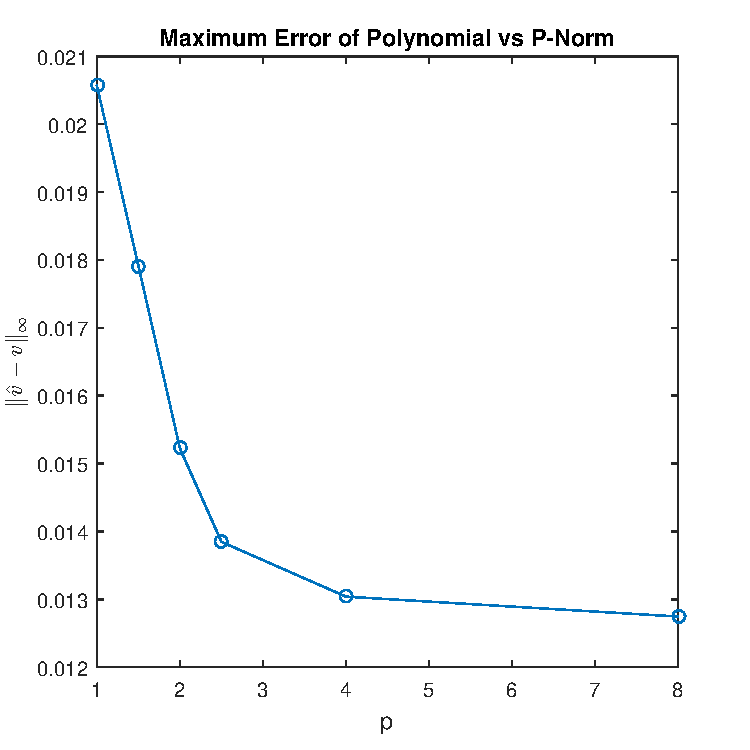
\includegraphics[height=0.35\textheight]{q11plot}
    \caption{Maximum Error vs P-Norm}
    \label{fig:q11}
\end{minipage}
\hspace{0.5cm}
\begin{minipage}[b]{0.45\linewidth}
    \centering
    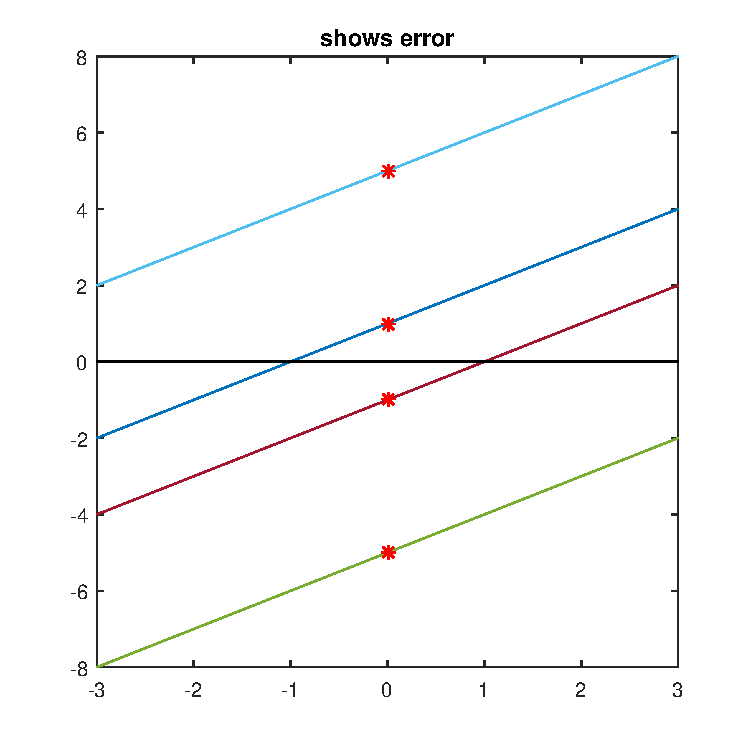
\includegraphics[height=0.35\textheight]{q12plot}
    \caption{CVX Line Optimization}
    \label{fig:q12}
\end{minipage}
\end{figure}


\section*{Question 13}

The obvious way to formulate the problem is shown by Equation \ref{eq:fac1}. 
\begin{equation}
\begin{aligned}
& \underset{x}{\text{minimize}}
& &\left\lVert{
      \begin{pmatrix}
      \|x-x_1\|_2 \\
      \|x-x_2\|_2 \\
      \cdots      \\
      \|x-x_N\|_2 \\
      \end{pmatrix}
    }\right\rVert_p\\
\end{aligned}
\label{eq:fac1}
\end{equation}

However, CVX requires the problem to be formulated in terms of inequalities in order to perform linear programming optimization. Equation \ref{eq:fac1} can be transformed into a linear system of inequalities as shown in Equation \ref{eq:fac2} where the RHS $y$ are added to the design variables.

A few examples have been plotted in Figure \ref{fig:fac}.

\begin{equation}
\begin{aligned}
& \underset{x,y}{\text{minimize}}
& &\|y\|_p \\
& \text{subject to}
& &\begin{pmatrix}
      \|x-x_1\|_2 \leq y_1 \\
      \|x-x_2\|_2 \leq y_2 \\
      \cdots               \\
      \|x-x_N\|_2 \leq y_N \\
   \end{pmatrix}\\
\end{aligned}
\label{eq:fac2}
\end{equation}


\begin{figure}[ht] 
  \begin{subfigure}[b]{0.5\linewidth}
    \centering
    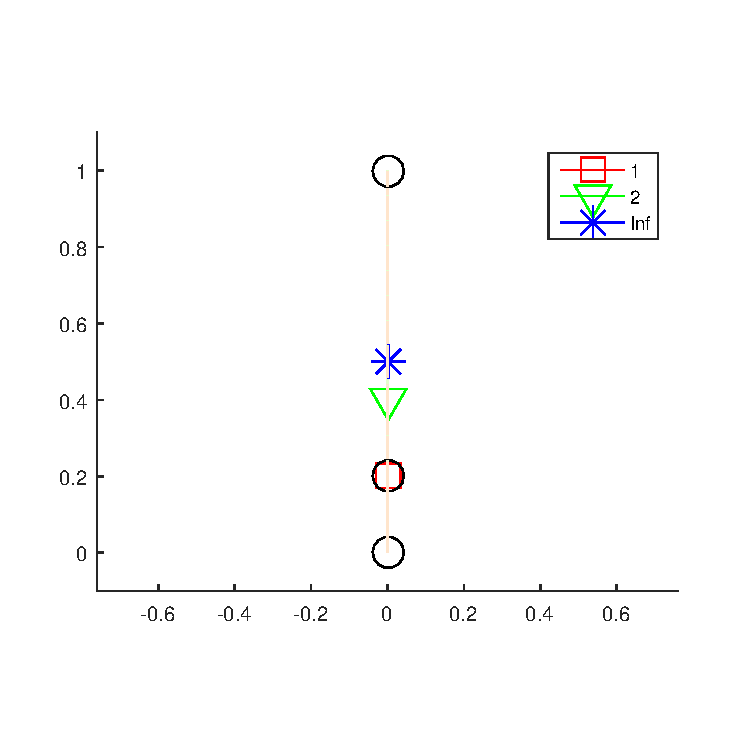
\includegraphics[width=0.9\linewidth]{fac4} 
  \end{subfigure}%% 
  \begin{subfigure}[b]{0.5\linewidth}
    \centering
    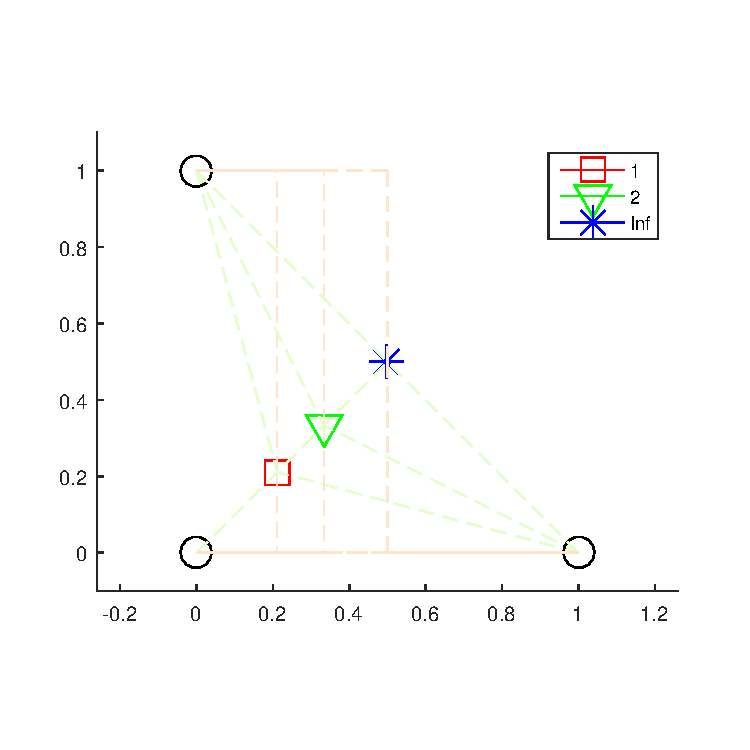
\includegraphics[width=0.9\linewidth]{fac1} 
  \end{subfigure} 
  \begin{subfigure}[b]{0.5\linewidth}
    \centering
    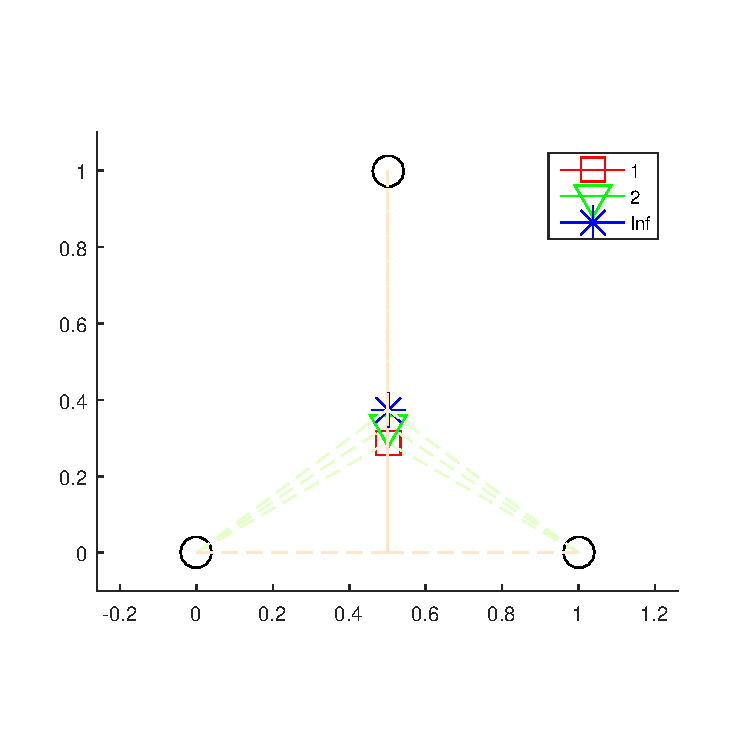
\includegraphics[width=0.9\linewidth]{fac2} 
  \end{subfigure}%%
  \begin{subfigure}[b]{0.5\linewidth}
    \centering
    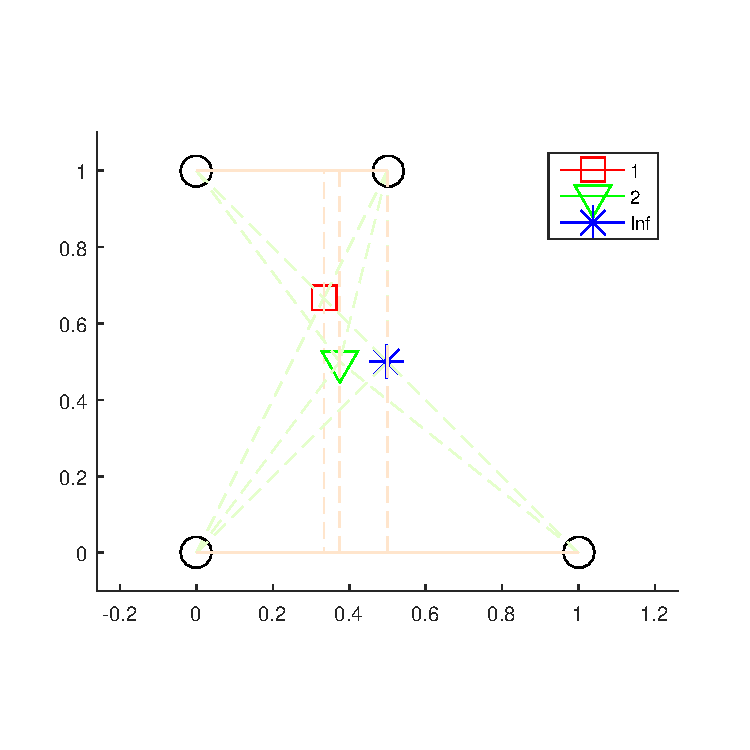
\includegraphics[width=0.9\linewidth]{fac3} 
  \end{subfigure} 
  \caption{Facility Location Results from CVX}
  \label{fig:fac} 
\end{figure}


\section*{Question 14}

Given two sets of point $U = \left\{u_1,\cdots,u_m\right\}$ and $V = \left\{v_1,\cdots,v_n\right\}$, we want a linear function $p(x) = c^T x -b$ which discriminates data. Once again, the problem is easily formulated into Equation \ref{eq:ld1}. 

\begin{equation}
\begin{aligned}
	 c^T u_i - b > 0 \quad & i=1,m\\
	 c^T v_i - b < 0 \quad & i=1,n\\
\end{aligned}
\label{eq:ld1}
\end{equation}

Since Equation \ref{eq:ld1} is a set of strict equalities and we require a set of inequalities, it is reformulated into Equation \ref{eq:ld2}. The new formulation maximizes the gap between the linear function and the set of points.

\begin{equation}
\begin{aligned}
& \underset{c,b,\delta}{\text{maximize}}
& & \delta \\
& \text{subject to}
& &	 c^T u_i - b \geq \delta \quad & i=1,m\\
&& &	 c^T v_i - b \leq -\delta \quad & i=1,n\\
\end{aligned}
\label{eq:ld2}
\end{equation}

The resulting line is plotted in figure \ref{fig:ld} with the following parameters:

\begin{equation*}
c^T = [148.3533, -157.4198] \quad b =-22.2961 \quad \delta = 1\\
\label{eq:ld3}
\end{equation*}

\begin{figure}[h]
    \centering
    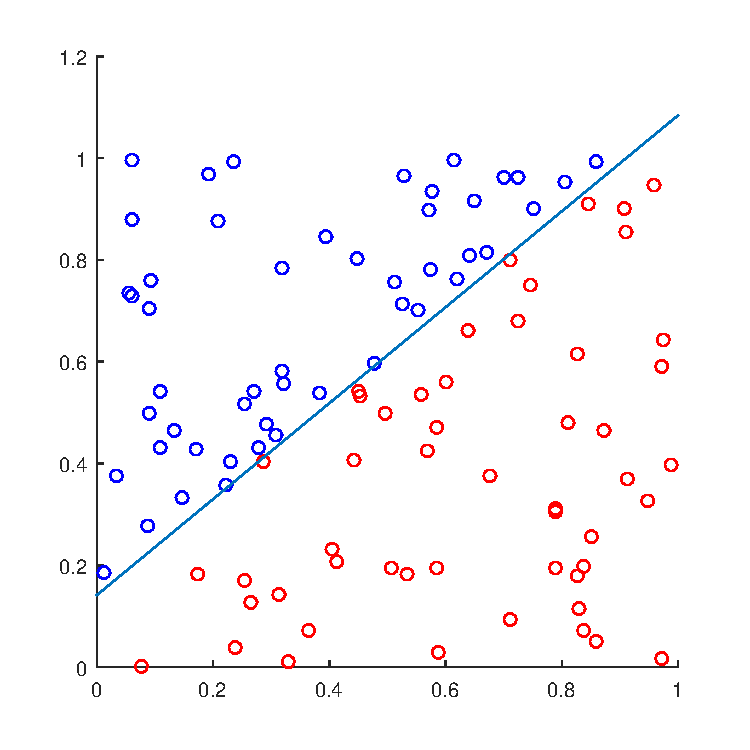
\includegraphics[height=0.35\textheight]{ld1}
    \caption{CVX Linear Discrimination}
    \label{fig:ld}
\end{figure}

\end{document}
